\lezione{24}{07.06.2017}
\section{Convergenza di variabili aleatorie}
\index{convergenza}
Lo studio delle \emph{successioni di variabili aleatorie} in probabilità è tanto importante quanto lo studio delle successioni numeriche e funzionali in analisi.
In particolare, si vuole studiare la loro \emph{convergenza} a un limite.
Nel caso delle variabili aleatorie esistono, in realtà, diverse definizioni di limite, e conseguentemente di convergenza, alcune più ``forti'' di altre.
In questo capitolo analizzeremo i principali tipi di convergenza, le loro proprietà, alcuni criteri e teoremi, il legame tra le varie convergenze, ed esempi e controesempi notevoli.

\begin{nb}
	I contenuti di questo capitolo e dei seguenti si estendono anche al caso in cui $X$ sia un vettore aleatorio e non una semplice variabile aleatoria (con una sola ovvia eccezione che sarà fatta notare al momento opportuno). Si è scelto di usare il caso in $\RR$ per semplicità di trattazione e di notazione.
\end{nb}

\medskip
Ricordiamo dall'analisi che una successione di funzioni $f_n: \RR^k \to \RR$ può convergere alla sua funzione limite $f: \RR^k \to \RR$ in due modi:
\begin{itemize}
    \item \textit{convergenza puntuale}, se $f_n(x) \xrightarrow{n} f(x) \ \forall \, x \in \RR^k$;
    \item \textit{convergenza uniforme}, se $\forall \varepsilon > 0 \enspace \exists \, n_0 = n_0(\varepsilon) \, : \, |f_n(x) - f(x)| < \varepsilon \enspace \forall x \in \RR^k \enspace \forall n \ge n_0$.
\end{itemize}

Per tutto il capitolo, sia $(\Omega, \Ac, \PP)$ lo spazio di probabilità su cui definiamo le variabili aleatorie $X_n: \Omega \to \RR$ e $X: \Omega \to \RR$.

\subsection{Convergenza certa e quasi certa}
\begin{defn}
  \index{convergenza!certa}
    La successione di VAR $X_n$ \textbf{converge certamente} a $X$
    se $X_n(\omega) \to X(\omega) \quad \forall \omega \in \Omega$.
\end{defn}

\begin{defn}
  \index{convergenza!quasi certa (qc)}
    La successione di VAR $X_n$ \textbf{converge quasi certamente} a $X$ (indicato con la notazione $X \xrightarrow{\text{qc}} X$) se l'evento $A = (X_n \to X)$ è tale che $A \in \Ac$ e $\PP(A) = 1$.
\end{defn}

\bigskip
\begin{ese} Alcune convergenze certe e quasi certe:
  \begin{itemize}
    \item Siano $f, f_n: \RR \to \RR$ funzioni continue, tali per cui $f_n$ converga puntualmente a $f$. \\
      Sia inoltre lo spazio di probabilità $\Omega = \RR, \Ac = \Bc, \PP = \Nc(0, 1)$, su cui si definiscono le variabili aleatorie $X_n(\omega) = f_n$ e $X(\omega) = f, \ \forall \omega \in \Omega$.\\
      Allora $X_n \to X$ certamente, e dunque anche quasi certamente. Si presti attenzione al fatto che le $X_n$ siano uguali alle $f_n$, non distribuite come le $f_n$.

    \item Sia $X_n = \Ind_{\left[0, \frac 1 n \right]}$. \\
      $X_n$ converge certamente a $X$, VA così definita:
      $$X = \begin{cases}
          0 &\text{per } \omega \neq 0 \\
          1 &\text{per } \omega = 0
      \end{cases}$$
      Inoltre, $X_n \xrightarrow{\text{qc}} 0$. Infatti, $X_n \to X$ per gli $\omega$ appartenenti ad $A = \RR_n \setminus \{ 0 \}$.

    \item Sia $X$ una VAR. Siano inoltre $X_n = \frac X n$.
      Allora $X_n \to 0$ certamente, e dunque anche quasi certamente.

    \item Sia $X \ge 0$ una VAR. \\
      Abbiamo già visto che è possibile costruire una successione di VA semplici tale per cui $X_n \uparrow X \ \forall \omega$. Questo è un caso di convergenza certa.

    \item Sia $X$ una VAR di legge $\Gc(P)$. Siano inoltre $X_n = X \wedge n = \min(X,n)$.
      Allora $X_n \xrightarrow{\text{qc}} X$.
  \end{itemize}
\end{ese}

Enunciamo ora alcune proprietà della convergenza quasi certa. Alcune sembreranno scontate, ma vedremo che non tutte varranno per gli altri tipi di convergenza.

\begin{prop}
  Siano le VAR $X_n, Y_n (\forall \, n), X$ e $Y$ tali che $X_n \xrightarrow{\text{qc}} X$, $Y_n \xrightarrow{\text{qc}} Y$. Siano inoltre $a \in \RR$ ed $h: \RR \to \RR$ funzione continua. Allora valgono le seguenti proprietà:
  \begin{enumerate}
    \item $a X_n \xrightarrow{\text{qc}} aX$
    \item $h(X_n) \xrightarrow{\text{qc}} h(X)$
    \item $X_n + Y_n \xrightarrow{\text{qc}} X + Y$
    \item $X_nY_n \xrightarrow{\text{qc}} XY$
    \item $Y, Y_n \neq 0 \ \forall \omega \implies \dfrac {X_n} {Y_n} \xrightarrow{\text{qc}} \dfrac X Y$
  \end{enumerate}
\end{prop}

\begin{dimo}
  Sarà dimostrato solo il punto (3). \\
  Per ipotesi, $X_n \xrightarrow{\text{qc}} X$ e $Y_n \xrightarrow{\text{qc}} Y$.
  Siano gli eventi $A_1 = (X_n \to X)$ e $A_2 = (Y_n \to Y)$.
  Per definizione di convergenza quasi certa, $\PP(A_1) = \PP(A_2) = 1$.

  Se $X_n$ e $Y_n$ convergono, necessariamente converge anche la loro somma\footnote{``Perché lo dice Verri''}: da questa condizione necessaria discende che
  $(X_n + Y_n \to X + Y) \supseteq A_1 \cap A_2$. \\
  Dunque $\PP(X_n + Y_n \to X + Y) \geq \PP(A_1, A_2) = 1$.
  Ma allora anche  $\PP(X_n + Y_n \to X + Y) = 1$ e vale la convergenza quasi certa.
\end{dimo}

\subsection{Convergenza in $L^p$}
\begin{defn}
  \index{convergenza!in $L^p$}
  La successione di VAR $X_n$ \textbf{converge in $L^p$} a $X$ ($X_n \xrightarrow{L^p} X$) se
  $X, X_n \in L^p$ e $\EE \left[ |X_n - X|^p \right] \to 0$.
\end{defn}

\vskip\smallskipamount
\begin{ese}
  Consideriamo le VA $X_n = \Ind_{\left[ 0, \frac 1 n \right]} \sim \Bc \left(\frac 1 n\right)$, definite su $\Omega = \RR, \ \Ac = \Bc, \ \PP = \Uc([0, 1])$. \\
  Allora $X_n \xrightarrow{L^1} 0$. Infatti $X_n \in L^1, 0 \in L^1, \Ex{|X_n - X|} = \Ex{|X_n|} = \frac 1 n \to 0$.
\end{ese}

\vskip\medskipamount
\begin{cese}[macchina da scrivere]\label{ese-macchina-scrivere}
  \index{macchina da scrivere}
  Si considerino le VAR $X_{jk} = \Ind_{\left[ \frac {j - 1} k; \frac j k \right]}$, con $k \in \NN$ e $1 \le j \le k$.

  Si faccia poi corrispondere a ogni $X_{jk}$ una $Y_i$, in modo da avere un solo indice: $X_{11} = Y_1, X_{12} = Y_2, X_{22} = Y_3, X_{13} = Y_4 \dots$

  $Y_n \xrightarrow{L^1} 0$, infatti $\Ex{|Y_n|} \to 0$; ma $Y_n \centernot{\xrightarrow{\text{qc}}} 0$. Anzi, $\liminf\limits_n Y_n = 0 $ e $\limsup\limits_n Y_n = 1, \ \forall \omega \in [0, 1]$: il limite della successione nemmeno esiste (perché i limiti inferiore e superiore non coincidono), men che meno c'è convergenza con probabilità $1$!
  \begin{figure}[H]
    \centering
    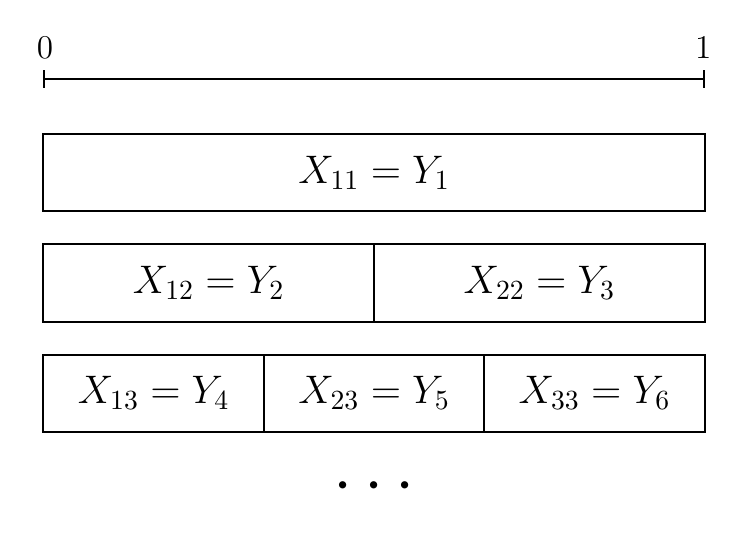
\begin{tikzpicture}[scale=1.4]
      \draw[|-|, line width=0.2mm] (0, 0.5) node[yshift=0.4cm, xshift=0.02cm] {\large $0$} -- (6, 0.5) node[yshift=0.4cm, xshift=-0.02cm] {\large $1$};
      \draw[line width=0.25mm] (0,0) rectangle (6, -0.7) node[pos=0.5] {\Large $X_{11} = Y_1$};
      \draw[line width=0.25mm] (0,-1) rectangle (3, -1.7) node[pos=0.5] {\Large $X_{12} = Y_2$};
      \draw[line width=0.25mm] (3,-1) rectangle (6, -1.7) node[pos=0.5] {\Large $X_{22} = Y_3$};
      \draw[line width=0.25mm] (0,-2) rectangle (2, -2.7) node[pos=0.5] {\Large $X_{13} = Y_4$};
      \draw[line width=0.25mm] (2,-2) rectangle (4, -2.7) node[pos=0.5] {\Large $X_{23} = Y_5$};
      \draw[line width=0.25mm] (4,-2) rectangle (6, -2.7) node[pos=0.5] {\Large $X_{33} = Y_6$};
      \node at (3,-3.2) {\Huge $\cdots$};
    \end{tikzpicture}
  \end{figure}
\end{cese}

\begin{prop}
  Siano le VAR $X_n \xrightarrow{L^p} X$, $Y_n \xrightarrow{L^p} Y$. Sia inoltre $a \in \RR$. Allora valgono le seguenti proprietà:
  \begin{enumerate}
    \item $a X_n \xrightarrow{L^p} aX$;
    \item $X_n + Y_n \xrightarrow{L^p} X + Y$;
    \item se $q \in [1,p]$, allora $\Ex{|X_n|^q} \xrightarrow{n} \Ex{|X|^q}$.
  \end{enumerate}
\end{prop}
Le due proprietà ``base'' di uno spazio vettoriale (somma e prodotto per scalare) sono garantite, il che è intuitivamente sensato, in quanto gli $L^p$ sono appunto spazi vettoriali.
Mancano tuttavia le proprietà di prodotto e rapporto. Sappiamo infatti che non è detto, per esempio, che il prodotto di due VA $L^1$ sia una VA $L^2$: mancando l'appartenenza a priori, non si può nemmeno parlare a priori di convergenza.

I casi più interessanti di applicazione delle proprietà sono la varianza e il valore atteso:
\begin{itemize}
	\item $p = 1 \implies \Ex{X_n} \xrightarrow{n} \Ex{X}$
	\item $p = 2 \implies \Ex{X_n} \xrightarrow{n} \Ex{X}, \enspace Var(X_n) \xrightarrow{L^p} Var(X)$
\end{itemize}

\begin{nb} Si ricorda che, presi $1 \le p \le q < +\infty$, gli spazi $L^p$ sono ``inscatolati'': $L^1 \supseteq L^p \supseteq L^q$.
\end{nb}

\subsection{Convergenza in probabilità}
\begin{defn}
  \index{convergenza!in probabilità ($\PP$)}
  La successione di VAR $X_n$ \textbf{converge in probabilità} a $X$ $(X_n \xrightarrow{\PP} X)$
  se $\forall \varepsilon > 0, \quad \PP(|X_n - X| > \varepsilon) \xrightarrow{n} 0$.
\end{defn}

\medskip
\begin{ese}
  Riprendiamo la macchina da scrivere.
  $Y_n \xrightarrow{\PP} 0$, poiché $\PP(|Y_n| > \varepsilon) = \PP(Y_n = 1) \xrightarrow{n} 0 \enspace \forall \varepsilon > 0$.
\end{ese}

\medskip
\begin{prop}
  Siano le VAR $X_n \xrightarrow{\PP} X, Y_n \xrightarrow{\PP} Y$. Siano inoltre $a \in \RR$ e $h: \RR \to \RR$ funzione continua. Allora valgono le seguenti proprietà:
  \begin{enumerate}
    \item $a X_n \xrightarrow{\PP} aX$
    \item $h(X_n) \xrightarrow{\PP} h(X)$
    \item $X_n + Y_n \xrightarrow{\PP} X + Y$
    \item $X_n Y_n \xrightarrow{\PP} XY$
    \item $Y, Y_n \neq 0 \ \forall \omega \implies \dfrac {X_n} {Y_n} \xrightarrow{\PP} \dfrac X Y$
  \end{enumerate}
\end{prop}
Si noti che sono le stesse 5 proprietà della convergenza quasi certa.

\begin{teob}[\JPTh{17.1}]
  $X_n$ converge in probabilità a $X \iff \EE \left[\dfrac {|X_n - X|} {1 + |X_n - X|} \right] \to 0$.
\end{teob}

\bigskip
\begin{dimo}
  Sia $\varepsilon > 0$ fissato e $X = 0$ senza perdita di generalità (infatti grazie alla proprietà (3) si può considerare la successione $Y_k \coloneqq X_n - X \to 0$: la tesi per $X=0$ equivale dunque alla tesi per $X$ generica).

  \begin{itemize}
    \item ($\implies$): ricordando che $\dfrac{|x|}{1+|x|} \leq 1 \ \ \forall x$ e che $\dfrac{|x|}{1+|x|} \leq \varepsilon \ \ \forall x : |x| \leq \varepsilon$, si può scrivere:
    \begin{align*}
      \dfrac {|X_n|} {1 + |X_n|} \
      &=\ \dfrac {|X_n|} {1 + |X_n|} \underbrace{(\Ind_{\{|X_n| > \varepsilon\}} + \Ind_{\{|X_n| \leq \varepsilon\}} )}_{=1} \\[6pt]
      &\le 1 \cdot \dfrac {|X_n|} {1 + |X_n|} \Ind_{\{|X_n| > \varepsilon\}} + \varepsilon \cdot \Ind_{\{|X_n| < \varepsilon\}} \\
      &\le\ \Ind_{\{|X_n| > \varepsilon\}} + \varepsilon \cdot 1
    \end{align*}
    Passando al valore atteso:
    $$\Ex{\dfrac {|X_n|} {1 + |X_n|}} \le \underbrace{\PP(|X_n| > \varepsilon)}_{\to 0 \text{ per hp}} + \varepsilon \implies
      \limsup_n \Ex{\dfrac {|X_n|} {1 + |X_n|}} \le \varepsilon \ \forall \varepsilon > 0$$
    Quindi, per definizione di convergenza, abbiamo la tesi:
    $$\Ex{\dfrac {|X_n|} {1 + |X_n|}} \to 0$$
    Infatti $\Ex{\dfrac {|X_n|} {1 + |X_n|}}$ è una VA sempre non negativa.
    \vskip\medskipamount

    \item ($\impliedby$): Si può scrivere che:
      $$\dfrac \varepsilon {1 + \varepsilon} \, \Ind_{\{|X_n| > \varepsilon\}} \ \le\ \dfrac {|X_n|} {1 + |X_n|} \Ind_{\{|X_n| > \varepsilon\}} \ \le\ \dfrac {|X_n|} {1 + |X_n|}$$
    Quindi, passando al valore atteso:
    $$\dfrac \varepsilon {1 + \varepsilon} \, \PP({|X_n| > \varepsilon}) \ \le\ \Ex{\dfrac {|X_n|} {1 + |X_n|}} \ \to 0 \implies \PP({|X_n| > \varepsilon}) \to 0 \enspace \forall \varepsilon > 0$$
    La tesi è dunque dimostrata. \qedhere
  \end{itemize}
\end{dimo}

\needspace{4\baselineskip}
\subsection{Relazioni tra tipi di convergenza (1)}
\begin{teob}[\JPTh{17.2}]\label{prop-rel-conv}
  \Fixvmode
  \begin{enumerate}
    \item $X_n \stackrel{qc}{\longrightarrow} X  \implies X_n \stackrel{\PP}{\longrightarrow} X$
    \item $X_n \stackrel{L^p}{\longrightarrow} X \implies X_n \stackrel{\PP}{\longrightarrow} X$
    \item $X_n \stackrel{L^q}{\longrightarrow} X \implies X_n \stackrel{L^p}{\longrightarrow} X, \ $ per $ 1 \le p \le q < +\infty$
  \end{enumerate}
\end{teob}
Si noti che per il punto (1) non vale l'implicazione inversa: si veda come controesempio la macchina da scrivere (pagina \pageref{ese-macchina-scrivere}).
Similmente, esistono controesempi in cui $ \int \lim \ne \lim \int$ che smentiscono il viceversa del punto (2).

\begin{dimo}
  \Fixvmode
  \begin{enumerate}
    \item $X_n - X \to 0$. Allora si può applicare la funzione continua $h(x)$ così definita:
      $$h(x) = \dfrac {\abs x} {1 + \abs x} \implies \dfrac {|X_n - X|} {1 + |X_n - X|} \xrightarrow{qc} 0 $$
      Si ha inoltre $\dfrac {|X_n - X|} {1 + |X_n - X|} \le 1 \in L^1$. Allora, per convergenza dominata:
      $$\Ex{\dfrac {|X_n - X|} {1 + |X_n - X|}} \to 0$$

    \item Fissato $\varepsilon > 0$, si ha:
      $$\PP(|X_n - X| > \varepsilon) \ =\ \PP(|X_n - X|^p > \varepsilon\,^p) \ \le\ \PP(|X_n - X|^p \ge \varepsilon\,^p)$$
      Applicando la disuguaglianza di Markov (teorema \ref{markov}), si trova:
      $$\PP(|X_n - X|^p \ge \varepsilon\,^p) \ \le\ \dfrac {\Ex{|X_n - X|^p}} {\varepsilon\,^p}\ \to\ 0$$

    \item La dimostrazione di questo punto richiede conoscenze avanzate, che lo studente più motivato apprenderà in corsi successivi. \qedhere
  \end{enumerate}
\end{dimo}
\Fixvmode

\begin{teob}[\JPTh{17.3}]\label{teo-conv-prob-qc}
  Se $X_n$ converge in probabilità a $X$, allora esiste una successione numerica $n_k$, cui corrisponde una sottosuccessione di VA $X_{n_k}$, tale che $X_{n_k} \xrightarrow{\text{qc}} X$.
\end{teob}

\medskip

\begin{dimo}
  Per ipotesi, $X_n \xrightarrow{\PP} X$, e dunque:
  $$\Ex{\dfrac {|X_n - X|} {1 + |X_n - X|}} \to 0$$
  Ma allora esiste una sottosuccessione $X_{n_k}$ tale per cui:
  $$\Ex{\dfrac {|X_{n_k} - X|} {1 + |X_{n_k} - X|}} \le \dfrac 1 {2^k}$$

  Consideriamo allora il valore atteso della somma. Poiché i termini sono positivi, si ha:
  $$\Ex{\sum\limits_{k=1}^{+\infty} \, \dfrac{|X_{n_k} - X|} {1 + |X_{n_k} - X|}} = \sum\limits_{k=1}^{+\infty} \, \Ex{\dfrac {|X_{n_k} - X|} {1 + |X_{n_k} - X|}} \le \sum\limits_{k=1}^{+\infty} \dfrac 1 {2^k} < +\infty$$

  Poiché il valore atteso della somma converge:
  $$\sum\limits_{k=1}^{+\infty} \dfrac{|X_{n_k} - X|} {1 + |X_{n_k} - X|} \stackrel{\text{qc}}{<} +\infty$$

  Allora $\dfrac{|X_{n_k} - X|} {1 + |X_{n_k} - X|} \xrightarrow{\text{qc}} 0$, da cui $|X_{n_k} - X| \xrightarrow{\text{qc}} 0$, e infine $X_{n_k} \xrightarrow{\text{qc}} X$.
\end{dimo}

\medskip
\textit{Esercizio.} Si applichi il teorema appena dimostrato all'esempio della macchina da scrivere. \\
Si prenda la sottosuccessione di VA $X_{11},X_{22}, X_{33},\dots$, che corrisponde all'ultima $X_{jk}$ per ogni riga $k$. Essa converge a $\Ind_{ \{ 1 \}}(\omega)$, ovvero a $1$ se l'esito elementare $\omega$ è proprio $1$ e a $0$ altrove. Inoltre si noti che $\Ind_{ \{ 1 \}}(\omega) = 0$ quasi certamente: dunque, $X_{nn} \xrightarrow{\text{qc}} 0$.  La successione in questione è $X_{nn}$ con $n \in \NN$, ovvero $Y_{n_k}$ con $n_k = \frac{n(n+1)} 2$ (si può facilmente verificare che i numeri $1,3,6,\dots$ di $n_k$ sono tutti numeri triangolari).

\vskip\bigskipamount
\begin{teob}[\JPTh{17.4}]\label{teo-conv-prob-lp}
  Siano le VAR $X_n, X, Y$ tali per cui: $X_n \stackrel{\PP}{\longrightarrow} X $, $\ |X_n| \le Y$ qc $\ \forall n$ e $\ Y \in L^p$ con $1 \le p < +\infty$. Allora:
  $$ \abs X \in L^p \quad \text{e} \quad X_n \stackrel{L^p}{\longrightarrow} X$$
\end{teob}

\lezione{25}{08.06.2017}

\begin{teo}[unicità del limite]
	Sia $X_n$ una successione di VAR, e siano $X$ e $\widetilde{X}$ VAR tali che $X_n\to X$ e $ X_n \to \widetilde{X}$, sia essa convergenza quasi certa, in $L^p$ o in probabilità. Allora $\widetilde X \aceq X$.
\end{teo}
\begin{dimo}
	Prendiamo il caso della convergenza quasi certa.
	Per definizione, dati $A, \widetilde A \in \Ac$ eventi quasi certi, si ha che:
	$$X_n(\omega) \to X(\omega) \ \forall \omega \in A \quad \text e \quad
	X_n(\omega) \to \widetilde X (\omega) \ \forall \omega \in \widetilde A$$
	Si definisca $A_0 = A \cap \widetilde A \in \Ac$, che è anch'esso un evento quasi certo.
	Pertanto:
	$$X_n(\omega) \to X(\omega) \quad \text e \quad X_n(\omega) \to \widetilde X(\omega) \ \forall \omega \in A_0$$
	Per l'unicità del limite puntuale, si ha che $X(\omega) = \widetilde X(\omega) \ \forall \omega \in A_0$, il quale è un evento quasi certo. \\
	La dimostrazione per gli altri tipi di convergenza è una semplice conseguenza del caso trattato.
\end{dimo}


\subsection{Convergenza in legge}
Si vuole spostare l'attenzione dai valori delle VA, osservati misurando per esempio $|X_n - X|$, alle loro leggi: che relazione c'è tra $P^{X_n}$ e $P^X$?

\begin{defn}
  \index{convergenza!debole}
  Siano $\PP_n$ e $\PP$ probabilità su $(\RR, \Bc)$. Si dice che \textbf{$\PP_n$ converge debolmente} a $\PP \ $ ($\PP_n \stackrel{\text{deb}}{\longrightarrow} \PP$) se:
  $$\int_\RR h \ \dPP_n \stackrel{n}{\longrightarrow} \int_\RR h \ \dPP \quad \forall h: \RR\to \RR \text{ continua e limitata}$$
\end{defn}

La condizione di limitatezza di $h$ serve semplicemente a garantire la convergenza dell'integrale a prescindere dalla probabilità considerata.
Di gran lunga più significativa è invece la richiesta di continuità della $h$, della cui utilità forniremo ora un esempio:

\smallskip
\begin{prop}
  Sia $x_n$ una successione numerica reale tale che $x_n\to x \in \RR$.
  Allora $\delta_{x_n} \stackrel{n}{\longrightarrow} \delta_x$ debolmente.
\end{prop}

\begin{dimo}
  Sia $h$ funzione qualsiasi continua e limitata. Allora:
  $$\lim_{n \to +\infty} \, \int_\RR h \ d \delta_{x_n} = \lim_{n \to +\infty} \,  h(x_n) = h\left(\lim_{n \to +\infty} x_n\right) = h(x) = \int_\RR h \ d \delta_x \qedhere$$
\end{dimo}

Come si può osservare, la continuità è necessaria per permettere lo scambio di limiti (quello di $n$ e l'integrale) che rappresenta la definizione di convergenza debole; non basta dunque $h$ solo misurabile per garantire tale convergenza sulla più semplice delle densità.

\smallskip
\begin{cese}
  Cerchiamo una $x_n$ successione numerica reale e $h$ misurabile e limitata (ma non continua) tali che $x_n \to x$ ma $\int_\RR h \ d \delta_{x_n} \centernot\to \int_\RR h \ d \delta_x$.
  Un possibile controesempio è dato da $x_n = \frac 1 n\to 0 = x$ con $h(t) = \Ind_{ (t = 0) }$ che è misurabile in quanto indicatrice: infatti $h(x_n) = 0 \ \forall n$ e $h(x_n) \centernot\to h(x) = 1$.
\end{cese}

\medskip
\begin{defn}
  \index{convergenza!in legge ($\Lc$)}
  Siano $X_n$ e $X$ VAR. Si dice che \textbf{$X_n$ converge in legge} o in distribuzione a $X \, $  ($X_n \stackrel{\Lc}{\longrightarrow} X$) se $P^{X_n}\xrightarrow{\text{deb}} P^X$.
\end{defn}

Si noti che la convergenza in legge è una \emph{relazione tra leggi} e solo tra leggi: non indica alcun legame tra i valori delle variabili aleatorie, bensì solo sulla loro probabilità.
Per evidenziare ciò, spesso si indica $P^X$ al posto di $X$ nella scrittura del limite.
Per esempio, se $X \sim \Nc(0,1)$, si scriverà $X_n \stackrel{\Lc}{\longrightarrow} \Nc(0,1) $.

\medskip
\begin{teob}[\JPTh{18.1}]
  $$X_n\to X \text{ in legge} \iff \EE_n[h(X_n)]\to \Ex{h(X)} \quad \forall h:\RR\to \RR \text{ continua e limitata}$$
\end{teob}

\begin{dimo}
  \Fixvmode
  \begin{align*}
    X_n \stackrel{\Lc}{\longrightarrow} X
    & \iff P^{X_n} \stackrel{deb}{\longrightarrow} P^X
    \iff \int_\RR h \ dP^{X_n}\to \int_\RR h \ dP^{X}\\
    & \iff \EE_n[h(X_n)]\to \Ex{h(X)} \ \forall h \text{ cont. e lim.}
  \end{align*}
  L'ultimo passaggio vale per la regola del valore atteso.
\end{dimo}

Si noti che la coimplicazione tra la scrittura con il simbolo di integrale e quella del valore atteso sembra una ridondanza, ma in realtà esse esprimono due concetti differenti. Nell'integrale la funzione integranda è sempre la stessa e cambia invece la probabilità che ``agisce'' su di essa; invece nel valore atteso è la funzione $h$ a cambiare valore e a convergere.

\medskip
\begin{nb} A differenza degli altri limiti (incluso quello della convergenza debole), il \emph{limite in legge \emph{non} è unico};
  ovvero, se $X_n$ converge in legge a due variabili $X$ e $\widetilde{X}$ si può concludere che $P^X = P^{\tilde X}$, ma \emph{non} che $X = \widetilde X$, nemmeno qc.
  Ancora una volta, distinguere tra convergenza di leggi di VA e convergenza di valori di VA è fondamentale.
\end{nb}

\subsection{Criteri di convergenza in legge}
\subsubsection{Caso discreto}
\begin{prop}
  Siano $X_n$ e $X$ VAR discrete, e sia $S = S_X \cup \left(\bigcup\limits_{n=1}^{+\infty}S_n\right)$ l'unione dei loro supporti, al più numerabile. Allora:
  $$ X_n \stackrel{\Lc}{\longrightarrow} X \iff \PP(X_n = s)\to \PP(X = s) \quad \forall s \in S$$
\end{prop}

\medskip
\begin{ese}[binomiale $\to$ Poisson] \ \\
  Siano $X_n \sim Bi\left(n, \frac \lambda n\right)$, con $n \geq \lambda > 0$, e $X \sim Po(\lambda)$.
  Il supporto è:
  $$S_{X_n} = \{ 0,\dots,n \} \ \forall n, \ S_X = \{ 0,1,\dots \} \implies S = \{ 0,1,\dots \}$$
  Fissando $k \in S$, si ha che:
  $$ \PP(X_n = k) =
  \begin{cases}
  0 & \text{per } n < k \\
  \binom n k p^k (1-p)^{n-k} & \text{per } n \geq k
  \end{cases}$$

  Per $n\to +\infty$ il primo caso non si verificherà più (ovvero si verificherà con probabilità nulla): calcolando $\lim\limits_{n \to +\infty} \PP(X_n = k)$ si ottiene, $\forall k \in S$, che:
  \begin{align*}
  \lim\limits_{n \to +\infty} &\frac{n!}{k!(n-k)!} \left(\frac \lambda n\right)^k \left(1 - \frac \lambda n\right)^{n-k} \\
  &=\frac {\lambda^k} {k!} \lim\limits_{n \to +\infty} \underbrace{\frac{n(n-1)\dots(n-k+1)}{n^k}}_{\to\ 1}
  \underbrace{\left( 1 - \frac \lambda n \right)^n}_{\to\ e^{-\lambda}}
  \underbrace{\left( 1 - \frac \lambda n \right)^{-k}}_{\to\ 1} = e^{-\lambda} \frac {\lambda^k}{k!}
  \end{align*}
  Dunque $X_n \stackrel{\Lc}{\longrightarrow} X$, ovvero:
  $$ X_n \text{ iid } Bi\left( n, \frac \lambda n \right) \implies \ X_n \stackrel{\Lc}{\longrightarrow} Po(\lambda)$$
\end{ese}

\subsubsection{Caso continuo}
\begin{teob}[\JPTh{18.5}]
  Siano $X_n, X$ VAR continue di densità continue rispettivamente $f_n$ e $f$.
  Allora:
  $$f_n \to f \text{ qo\footnotemark} \implies X_n \xrightarrow{\Lc} X$$
  \footnotetext{Ricordiamo che ``quasi ovunque'' significa ``convergenza puntuale tranne eventualmente in insiemi di misura di Lebesgue nulla''. Se a pagina \thepage $ $ non avete ancora capito il concetto di ``quasi ovunque'' potrebbe essere un problema.}
\end{teob}

\medskip
\begin{ese}
  $\Nc \to \Nc$. \\
  Siano $X_n \sim \Nc(\mu,\sigma_n^2)$ tali che, $\sigma_n^2 > 0 \ \forall n, \mu_n \to \mu$ e $\sigma_n^2 \to \sigma^2 > 0$. Per definizione:
  $$f_n(s) = \frac 1 {\sqrt{2 \pi \sigma_n^2}} \exp\left\{ \frac{-(s-\mu_n)^2}{2\sigma_n^2} \right\}$$
  Per $n$ che tende ad infinito e data una $f_n$ continua, allora:
  $$f_n(s) \xrightarrow[f_n \text{ cont.}]{n} \frac 1 {\sqrt{2 \pi \sigma^2}} \exp\left\{ \frac{-(s-\mu)^2}{2\sigma^2} \right\} = f(s) \quad \forall s \in \RR = S$$
  Ovvero, riassumendo:
  $$ X_n \sim \Nc(\mu_n,\sigma_n^2) \ \implies \ X_n \stackrel{\Lc}{\longrightarrow} \Nc(\mu,\sigma^2) $$
  Da ciò consegue, per definizione di convergenza in legge, che, $\forall h$ continua e limitata:
  $$ \int_\RR h(s) \frac 1 {\sqrt{2 \pi \sigma_n^2}} \exp\left\{ \frac{-(s-\mu_n)^2}{2\sigma_n^2} \right\} \de s \overset{n}{\longrightarrow}
  \int_\RR h(s)  \frac 1 {\sqrt{2 \pi \sigma^2}} \exp\left\{ \frac{-(s-\mu)^2}{2\sigma^2} \right\} \de s$$
  Abbiamo, di fatto, lo scambio dei limiti anche senza aver invocato la convergenza monotona o dominata; esse sono infatti condizioni solo sufficienti, e non necessarie, per lo scambio.
\end{ese}

In generale, se $X_n \stackrel{\Lc}{\longrightarrow} X$, \emph{non} si può dedurre che $\PP(X_n \in B) \to \PP(X \in B)$ con $B \in \Bc$, che $\Ex{X_n} \to \Ex X$ o che $Var(X_n) \to Var(X)$.


\textit{Esercizio.} Trovare controesempi per le ultime due affermazioni.

\subsubsection{Caso generale: funzione di ripartizione}
\begin{teob}[\JPTh{18.4}]
  Siano $X_n$ e $X$ VAR con funzione di ripartizione $F_n$ e $F$, rispettivamente. \\
  Allora, $\forall s \in \RR$ in cui $F$ è continua, ovvero esclusi eventualmente i salti di $F$:
  $$ X_n \stackrel{\Lc}{\longrightarrow} X \iff F_n(s) \to F(s)$$
  Quindi, se $X$ è continua (e dunque anche $F$ è continua), allora $\PP(X_n \in B) \to \PP(X \in B) \enspace \forall B \in \Bc$.
\end{teob}
Questa proprietà \emph{non} è valida per i vettori aleatori in $\RR^n$, visto che in spazi di dimensione maggiore di 1 la funzione di ripartizione diventa un oggetto più complicato da studiare e da utilizzare.

\medskip
\begin{ese} Continua $\to$ discreta. \\
  Siano $X_n \sim U \left( \left[ -\frac 1 n, \frac 1 n \right] \right)$. L'intuizione suggerisce che $X_n$ convergerà a una legge massa (discreta). \\
  Calcolare le funzioni di ripartizione delle VA consentirà di studiarne la convergenza in legge:
  $$ F_n(s) =
  \begin{cases}
    0 & \text{ per } s \leq -\frac 1 n \\
    \frac 1 2 - \frac n 2 s & \text{ per } -\frac 1 n < s \leq \frac 1 n\\
    1 & \text{ per } s > \frac 1 n
  \end{cases}
  \overset{n}{\longrightarrow}
  \begin{cases}
    0 & \text{ per } s < 0 \\
    \frac 1 2 & \text{ per } s = 0 \\
    1 & \text{ per } s > 0
  \end{cases}
  \overset{\text{qo}}{=} \Ind_{[0,+\infty]}(s) = F_{\delta_0}(s)$$
  Ovvero:
  $$ X_n \sim U \left( \left[ -\frac 1 n, \frac 1 n \right] \right) \implies
  X_n \stackrel{\Lc}{\longrightarrow} \delta_0$$
  Tale risultato si può anche scrivere come $X_n \stackrel{\Lc}{\longrightarrow} X$ con $X \sim \delta_0$, come $X \aceq 0$ o come $X_n \stackrel{\Lc}{\longrightarrow} 0$.
  \begin{figure}[H]

    \centering
    \(
    \vcenter{\hbox{\begin{tikzpicture}
    \begin{axis}[
    axis lines = middle,
    width=0.45\textwidth,
    yticklabels={,,},
    xticklabels={,,}
    ]

    \draw [line width=0.4mm, color=lightblue] (axis cs:-2,0) -- (axis cs:-1,0) -- (axis cs:-1,2)-- (axis cs:1,2) -- (axis cs:1,0)-- (axis cs:2,0);


    \addplot [draw=none, forget plot] coordinates {(-2,3)};
    \addplot [draw=none, forget plot] coordinates {(2,-1)};

    \addplot [draw=none, forget plot] coordinates {(-1,0)} node[below] {$-\frac{1}{n}$};
    \addplot [draw=none, forget plot] coordinates {(1,0)} node[below] {$\frac{1}{n}$};
    \addplot [draw=none, forget plot] coordinates {(0,2)} node[below left] {$\frac{n}{2}$};

    \end{axis}
    \end{tikzpicture}}}
    \)
    \hskip 5pt
    $\longrightarrow$
    \hskip 5pt
    \(
    \vcenter{\hbox{\begin{tikzpicture}
    \begin{axis}[
    axis lines = middle,
    width=0.45\textwidth,
    yticklabels={,,},
    xticklabels={,,}
    ]

    \draw [line width=0.4mm, color=lightblue] (axis cs:-2,0) -- (axis cs:0,0) -- (axis cs:0,3)-- (axis cs:0,0) -- (axis cs:2,0);

    \addplot [draw=none, forget plot] coordinates {(-2,3)};
    \addplot [draw=none, forget plot] coordinates {(2,-1)};

    \end{axis}
    \end{tikzpicture}}}
    \)
    \hskip 20pt
    \(
    \vcenter{\hbox{\begin{tikzpicture}
    \begin{axis}[
    axis lines = middle,
    xlabel = $s$,
    ylabel = $F_n(s)$,
    width=0.45\textwidth,
    yticklabels={,,},
    xticklabels={,,}
    ]

    \draw [line width=0.4mm, color=lightblue] (axis cs:-2,0) -- (axis cs:-1,0) -- (axis cs:1,2) -- (axis cs:2,2);
    \draw [line width=0.1mm, dashed] (axis cs:0,2) -- (axis cs:1,2);

    \addplot [draw=none, forget plot] coordinates {(-2,3)};
    \addplot [draw=none, forget plot] coordinates {(2,-1)};

    \addplot [draw=none, forget plot] coordinates {(-1,0)} node[below] {$-\frac{1}{n}$};
    \addplot [draw=none, forget plot] coordinates {(1,0)} node[below] {$\frac{1}{n}$};
    \addplot [draw=none, forget plot] coordinates {(0,2)} node[left] {$1$};

    \end{axis}
    \end{tikzpicture}}}
    \)
    \hskip 5pt
    $\longrightarrow$
    \hskip 5pt
    \(
    \vcenter{\hbox{\begin{tikzpicture}
    \begin{axis}[
    axis lines = middle,
    xlabel = $s$,
    ylabel = $F_n(s)$,
    width=0.45\textwidth,
    yticklabels={,,},
    xticklabels={,,}
    ]

    \draw [line width=0.4mm, color=lightblue] (axis cs:-2,0) -- (axis cs:0,0) -- (axis cs:0,2) -- (axis cs:2,2);


    \addplot [draw=none, forget plot] coordinates {(-2,3)};
    \addplot [draw=none, forget plot] coordinates {(2,-1)};

    \addplot [draw=none, forget plot] coordinates {(0,2)} node[left] {$1$};

    \end{axis}
    \end{tikzpicture}}}
    \)
    \caption{distribuzione e funzione di ripartizione da uniforme continua a delta discreta} \label{plot-conv}
  \end{figure}
\end{ese}

\begin{ese} Discreta $\to$ continua. \\
  Siano $X_n \sim U(A)$, con $A = \left\{\frac 1 n, \frac 2 n, \dots, 1\right\}$. L'intuizione suggerisce che $X_n$ convergerà a una legge uniforme sull'intervallo $[0,1]$ (continua). \\
  Come già nell'esempio precedente, operiamo sulle funzioni di ripartizione. Si definisca quindi $F_n(s)$:
  $$F_n(s) =
  \begin{cases}
    0 & \text{ per } s \leq \frac 1 n \\
    \frac k n & \text{ per } \frac k n < s \leq \frac{k+1} n \ (k \in \NN, k \leq n) \\
    1 & \text{ per } s > 1
  \end{cases}$$
  Prendendo il limite su $n$:
  $$F_n(s) \xrightarrow{n \to +\infty}
  \begin{cases}
    0 & \text{ per } s \leq 0 \\
    s & \text{ per } 0 < s \leq 1 \\
    1 & \text{ per } s > 1
  \end{cases}
  = F_{X \sim {U([0,1])}}(s) = F(s)$$
  Ovvero, riassumendo:
  $$ X_n \sim U\left( \left\{ \frac 1 n, \dots, 1 \right\} \right) \implies
  X_n \xrightarrow[n]{\Lc} U([0,1])$$
  \begin{figure}[H]

    \centering
    \begin{tikzpicture}
    \begin{axis}[
    axis lines = middle,
    width=0.5\textwidth,
    xlabel = $s$,
    ylabel = $F_n(s)$,
    yticklabels={,,},
    xticklabels={,,}
    ]

    \draw [line width=0.3mm, color=lightblue] (axis cs:-1,0) -- (axis cs:1,0);
    \draw [line width=0.3mm, color=lightblue] (axis cs:1,1) -- (axis cs:2,1);
    \draw [line width=0.3mm, color=lightblue] (axis cs:2,2) -- (axis cs:3,2);
    \draw [line width=0.3mm, dashed, color=lightblue] (axis cs:3,3) -- (axis cs:4,3);
    \draw [line width=0.3mm, color=lightblue] (axis cs:4,4) -- (axis cs:5,4);

    \draw [line width=0.3mm, red, dashed] (axis cs:-1,0) -- (axis cs:0,0);
    \draw [line width=0.3mm, red, dashed] (axis cs:0,0) -- (axis cs:5,5);



    \draw [fill=lightblue] (axis cs:1,1)  circle (4);
    \draw [fill=lightblue] (axis cs:2,2)  circle (4);
    \draw [fill=lightblue] (axis cs:4,4)  circle (4);

    \addplot [draw=none, forget plot] coordinates {(1.45,0.35)} node {$45\degree$};

    \addplot [draw=none, forget plot] coordinates {(-1,-1)};
    \addplot [draw=none, forget plot] coordinates {(5,5)};

    \addplot [draw=none, forget plot] coordinates {(1,0)} node[below] {$\frac{1}{n}$};
    \addplot [draw=none, forget plot] coordinates {(2,0)} node[below] {$\frac{2}{n}$};
    \addplot [draw=none, forget plot] coordinates {(3,0)} node[below] {$\dots$};
    \addplot [draw=none, forget plot] coordinates {(4,0)} node[below] {$1$};

		\draw [black] (axis cs:1,0) arc[start angle=0, end angle=45,
                              			radius={transformdirectionx(1)}];
    \end{axis}

    \end{tikzpicture}

    \caption{intuizione del passaggio da discreto a continuo}\label{fig-intuizione-discreto-continuo}
  \end{figure}

  Per convincersi che un insieme discreto \emph{numerabile} converga su un insieme \emph{continuo}\footnote{No, seriamente, WTF?}, si osservi che:
  $$|F_n(s) - F(s)| = s - F(s) < \frac{k+1} n - \frac k n = \frac 1 n \to 0 \quad \forall s \in \RR$$
  Ovvero, l'errore tra le due funzioni si annulla per $n \to +\infty$.
  In alternativa, si osservi che:
  $$ \PP(a < X_n \leq b) = \frac{\#\{ k \in \NN | a < \frac k n \leq b \}}n \to b-a = \PP(a < X \leq b)$$
  Ovvero, la probabilità di un intervallo sulla uniforme discreta tende alla sua probabilità sull'uniforme continua.
\end{ese}

\subsubsection{Caso generale: funzione caratteristica}
È il caso più importante e utilizzato dei 4 menzionati finora.

\begin{teo}[continuità di Levy \JPTh{19.1}]
  \Fixvmode
  \index{Levy, teorema di continuità di}
  \begin{enumerate}
    \item Se $X_n \stackrel{\Lc}{\longrightarrow} X$, allora $\varphi_n(u) \to \varphi(u) \ \forall u \in \RR$.
    \item Siano $X_n$ VAR tali che $\varphi_n(u) \to \psi(u)$, con $\psi$ funzione generica ma continua in $0$.
    Allora $\exists X$ VAR avente $\psi$ come funzione caratteristica e tale che $X_n \stackrel{\Lc}{\longrightarrow} X$.
  \end{enumerate}
\end{teo}
Il punto (1) è una conseguenza dell'unicità della legge limite e della reciproca caratterizzazione tra una legge e la sua funzione caratteristica. L'intero teorema è sostanzialmente una coimplicazione tra convergenza in legge (``probabilistica'') delle VA e convergenza puntuale (``analitica'') delle rispettive funzioni caratteristiche.

Tuttavia per il punto (2) si richiedono ipotesi più semplici: non serve controllare che $\psi$ sia effettivamente una funzione caratteristica, basta che sia continua in 0.
A questo riguardo, si noti che se è verificata questa ipotesi allora necessariamente $\psi(0) = 1$ perché $\psi$ è la funzione limite delle $\varphi$, che hanno tutte valore 1 in 0.

\medskip
\begin{ese}
  Siano $X_n \sim \Nc(\mu_n,\sigma_n^2),
  \sigma^2 \geq 0, \mu_n \to \mu, \sigma_n^2 \to \sigma^2 \geq 0$.
  Per definizione, la funzione caratteristica è:
  $$ \varphi_n(u) = \exp\left\{ iu\mu_n - \frac 1 2 u^2 \sigma_n^2 \right\}$$
  Facendo tendere $n$ all'infinito e per $\varphi_n(u)$ continua in $\mu_n$ e $\sigma_n$:
  $$\varphi_n(u) \xrightarrow{n} \exp\left\{ iu\mu - \frac 1 2 u^2 \sigma^2 \right\} = \varphi_X(u) \text{ con } X \sim \Nc(\mu,\sigma^2)$$
  In altre parole:
  $$X_n \sim \Nc(\sigma_n, \mu_n^2) \implies X_n \stackrel{\Lc}{\longrightarrow} \Nc(\mu,\sigma^2)$$ \\
\end{ese}
\begin{nb}
  Se $\sigma^2 = 0$, allora $\Nc(\mu,\sigma^2) = \Nc(\mu,0) = \delta_\mu$, ovvero $X_n \stackrel\Lc{\longrightarrow} \mu$.
\end{nb}

\medskip
\begin{ese}
  Siano $X_n \sim Bi\left(n, \frac \lambda n\right)$ con $n \geq \lambda > 0$. Allora, per definizione:
  $$\varphi_n(u) = \left( e^{iu} \frac \lambda n + 1 - \frac \lambda n \right)^n = \left[ 1 + \frac 1 n \lambda \left(e^{iu}-1\right) \right]^n$$
  Prendendo il limite su $n$:
  $$\varphi_n(u) \stackrel{n}{\longrightarrow} exp \left\{ \lambda (e^{iu}-1) \right\} =
  \varphi_X(u) \text{ con } X \sim Po(\lambda)$$
  Ovvero, riassumendo: $$X_n \sim Bi\left(n, \frac \lambda n\right) \implies X_n \stackrel{\Lc}{\longrightarrow} Po(\lambda)$$
\end{ese}

\medskip
\begin{cese}
  La successione $X_n \sim U([-n,n])$ \emph{non} converge in legge, in quanto:
  $$\varphi_n(u) = \frac{\sin(nu)}{nu} \stackrel{n}{\longrightarrow}
  \begin{cases}
    1 & \text{per } u = 0 \\
    0 & \text{per } u \neq 0
  \end{cases}
  \ = \psi(u)$$
  $\psi(u)$ non è infatti continua in $u = 0$.
\end{cese}

\subsection{Relazioni tra tipi di convergenza (2)}
\begin{teob}[\JPTh{18.2}]
  Siano $X_n, X$ VAR tutte definite sullo stesso spazio di probabilità $\Dom$.
  Allora:
  $$X_n \xrightarrow{\PP} X \implies X_n \xrightarrow{\Lc} X$$
\end{teob}
Con questo teorema la convergenza in legge diventa la più ``debole'' tra i vari tipi di convergenza, perché è implicata dalla convergenza in probabilità che a sua volta era implicata da tutte le altre.

\begin{dimo}
  Poiché per ipotesi $X_n \stackrel{\PP}{\longrightarrow} X$, è anche vero che $h(X_n) \stackrel{\PP}{\longrightarrow} h(X)$ per tutte le $h$ continue, comprese quelle continue e anche limitate.
  In quest'ultimo caso, applicando la convergenza dominata si ottiene che $\Ex{h(X_n)} \to \Ex{h(X)} \ \forall h$ continua e limitata, ovvero, per definizione, $X_n \stackrel{\Lc}{\longrightarrow} X$.
\end{dimo}

Il viceversa \emph{non} è valido perché il limite in legge non è unico, tranne che nel seguente caso specifico:
\begin{teob}[\JPTh{18.3}]\label{conv-costante}
  Siano $X_n, X$ VAR tutte definite sullo stesso spazio di probabilità $\Dom$ e $c \in \RR$ una costante.
  Allora:
  $$X_n \stackrel{\Lc}{\longrightarrow} c \implies X_n \xrightarrow{\PP} c$$
\end{teob}

\begin{dimo}
  $X_n \stackrel{\Lc}{\longrightarrow} c, c \in \RR$ se e solo se
  $\Ex{h(X_n)} \to \Ex{h(c)} = h(c) \ \forall h$ continua e limitata.
  Scegliendo in particolare:
  $$h(x) = \frac{|x-c|}{1+|x-c|} \implies \Ex{ \frac{|X_n - c|}{1+|X_n - c|} } \to h(c) = 0$$
  Ovvero, per definizione, $X_n \stackrel\PP{\longrightarrow} c$.
\end{dimo}

\begin{prop}[proprietà della convergenza in legge]
  Siano $X_n, X, Y_n$ VAR tali che $X_n \stackrel{\Lc}{\longrightarrow} X$ e $Y_n \stackrel{\Lc}{\longrightarrow} c \in \RR, a \in \RR$, e $h:\RR \to \RR$ funzione continua.
  Allora:
  \begin{enumerate}
    \item[0.] $P^X$ è unica, come già sappiamo
    \item $a X_n \stackrel{\Lc}{\longrightarrow} aX$
    \item $h(X_n) \stackrel{\Lc}{\longrightarrow} h(X)$
  \end{enumerate}
  Vale inoltre il \emph{teorema di Slutsky}, riportato di seguito.
\end{prop}

\bigskip

\begin{teo}[teorema di Slutsky \JPTh{18.8}]\label{collegeslutsky}
  \index{Slutsky, teorema di}
  Nelle stesse ipotesi:
  \begin{enumerate}
    \item[3.] $X_n + Y_n \stackrel{\Lc}{\longrightarrow} X + c$.
    \item[4.] $X_n Y_n \stackrel{\Lc}{\longrightarrow} cX$.
    \item[5.] $Y_n, c \neq 0 \implies \frac{X_n}{Y_n} \stackrel{\Lc}{\longrightarrow} \frac 1 c X$.
  \end{enumerate}
\end{teo}
Si noti che nella coppia di variabili aleatorie descritta dal teorema di Slutsky, almeno una delle due converge in legge a una \emph{costante}: non potrebbe essere altrimenti, visto che l'eventuale legge di convergenza di una funzione di $X$ e $Y$ dipende anche dalle correlazioni tra $X$ e $Y$ (covarianza etc.), di cui non c'è menzione nelle ipotesi del teorema.

\subsubsection{Riepilogo delle relazioni fra convergenze}
\begin{figure}[H]
  \centering
  \includegraphics[width=0.5\textwidth]{img/schema_convergenza.png}
  \caption{schema riassuntivo dei teoremi sulle relazioni tra i teoremi della convergenza}
\end{figure}
\begin{itemize}
  \item La convergenza in probabilità ha una sottosuccessione che converge quasi certamente per il teorema \ref{teo-conv-prob-qc};
  \item Dati $p$ e $q$ con $p \geq q$, la convergenza in $L^p$ implica la convergenza in $L^q$ per la proposizione \ref{prop-rel-conv};
  \item Dati $|X| \in L^p$, $\ |X_n| \le Y$ qc $\ \forall n$ e $\ Y \in L^p$, ovvero rispettano una convergenza dominata e sono in $L^p$, allora è possibile, data la convergenza in probabilità, ottenere quella in $L^p$ come enunciato dal teorema \ref{teo-conv-prob-lp};
  \item Se $X_n$ converge ad una costante allora la convergenza in legge implica quella in probabilità, per il teorema \ref{conv-costante}.
\end{itemize}

\cleardoublepage
